\chapter{État de l’art}

\section{Le dérèglement climatique}

Nous pouvons faire l’analogie avec une application logicielle. Une règle courante est d’éviter
l’optimisation prématurée, c’est à dire de ne pas optimiser tant que le besoin ne s’en fait pas
ressentir. Nous risquerions de dépenser du temps et de l'énergie dans quelques chose qui
peut-être ne fonctionne pas comme nous le voudrions.
Dans un premier temps, il faut faire en sorte que le système fonctionne correctement.
On peut préférer la quantité face à la qualité. On ne cherche à optimiser cette méthode
qu’ensuite, lorsque les ressources commencent à ne plus suffire ou qu’un besoin de remise
à l’échelle se fait sentir.

Aujourd'hui nous sommes en mesure de produire suffisamment d’énergie pour répondre aux
besoin de la population. Mais le contexte environnementale nous impose désormais d’optimiser
nos méthodes : épuisement des énergies fossiles, réchauffement climatique, augmentation de la
population.

\section{Augmentation des besoins en énergie}

L'énergie apporte l'augmentation de la consommation d'énergie, comme le montre la figure
~\ref{fig:capita_energy}, chaque personne consomme plus d'énergie qu'un habitant
du début des années 1800.

\begin{SCfigure}[][h]
  \centering
  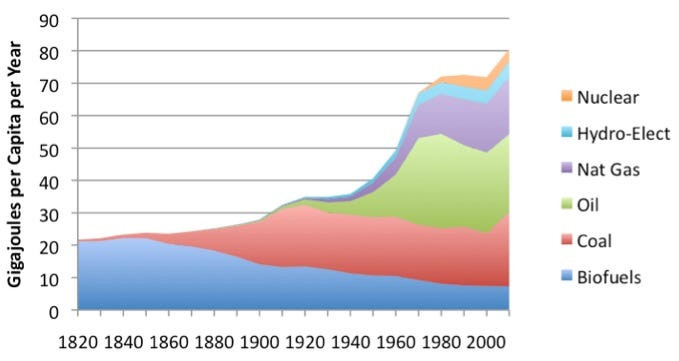
\includegraphics[scale=0.35]{media/world_per_capita_energy.jpeg}
  \caption{
      Consommation d'énergie par personne\newline
      \tiny{Source:\newline
        \url{https://www.businessinsider.com/a-worrying-look-at-world-energy-consumption-since-1820-2012-3?IR=T}
      }
  }
  \label{fig:capita_energy}
\end{SCfigure}

Cette augmentation de consommation d'énergie par habitant j'ajoute a une augmentation
massive de la population sur Terre.

\begin{SCfigure}[][h]
  \centering
  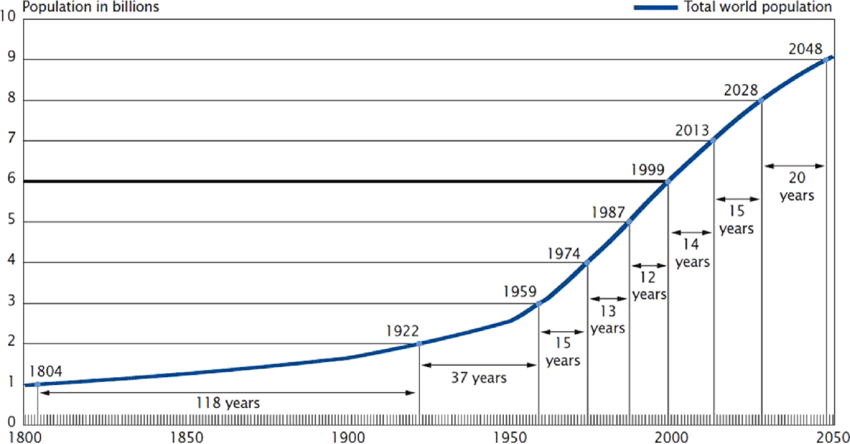
\includegraphics[scale=0.35]{media/WorldPopulation.png}
  \caption{
      Population sur Terre\newline
      \tiny{Source:\newline
        \url{https://www.researchgate.net/figure/World-Population-1800-2050-6_fig1_321996838}
      }
  }
  \label{fig:capita_energy}
\end{SCfigure}

\section{Guerre de l'énergie}
\section{Amélioration des performances informatique}
